% !TeX spellcheck = en_GB
\chapter{Load balancing}

When dealing with redundant distributed systems, there exists more than one node capable of doing some work.
In such a system the workload needs to be distributed and balanced across all nodes.
Load balancing for large systems can be split in tiers. The top tier being region based load balancing using DNS servers using knowledge of where the request was revived \cite{Amazon:Route53}. At a lower tier it could be machine level based on performance parameters like \cite{zhang2000linuxVirtualServer}, to application level based on the content of the request \cite{Citation is missing and I need to find it}. There exists a lot of solution specific load balancers.
A node balancer is a service witch distributes incoming requests, among the services registered on the network.
The distribution is based on different policies like dividing packages or picking the one with most free CPU capacity.
The load balancer could be a single point of failure, it should for this reason always have one or more backups as seen in \cref{fig:loadBalancingSetup}.
The load balancer monitors the real servers and only parses on requests to running servers.
A secondary needs to monitor the primary load balancer and step in if it stops responding. This can be done using a virtual private IP, which is the address for all incoming requests.

\begin{figure}
	\centering	
	\scalebox{0.7}{\begin{tikzpicture}[
	start chain=going right,
	diagram item/.style={
		minimum width=80pt,
%		minimum height=45pt,
		on chain,
		join
	},
	diagram item seperated/.style={
			minimum width=80pt,
	%		minimum height=45pt,
			on chain
		}
]
\node [
	diagram item,
  label=center:Internet
] (Internet) {
\includegraphics{Cisco_BW/cloud}};

%\node [
%	continue chain=going below,
%	diagram item,
%	label=right:Router
%] {
\includegraphics{Cisco_BW/router}};

\node [
	start branch=1 going below right,
	diagram item seperated,
	label={[align=center]right:Load\\Balancer\\(Secondary)}
] (LB2) {
\includegraphics{Cisco_BW/distributed_director}};

\node [
	continue chain=going below left,
	diagram item,
	label={[align=center]left:Load\\Balancer\\(Primary)}
] (LB1) {
\includegraphics{Cisco_BW/distributed_director}};

\node [
	continue chain = going below right,
	diagram item,
	label={[align=center]right:Services in distrinbuted\\across the wind farm}
] (farm) {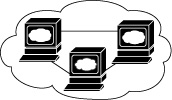
\includegraphics{Cisco_BW/web_cluster}};

\draw[loosely dotted] (LB1) -> (LB2) node[fill=white,midway]{heatbeat};
\draw[dashed] (Internet) -> (LB2);
\draw[dashed] (LB2) -> (farm);

\node [
	start branch=1 going below right,
	diagram item,
	label=below:Other interface
] {\includegraphics{Cisco_BW/PC}};

\node [
	start branch=1 going below left,
	diagram item,
	label=below:Http interface
] {\includegraphics{Cisco_BW/PC}};

\node [
	continue chain = going below,
	diagram item,
	label=below:Modbus interface
] {\includegraphics{Cisco_BW/PC}};

\end{tikzpicture}}
	\captionsetup{format=plain,font=footnotesize,labelfont={bf,defaultCapFont},labelsep=quad,singlelinecheck=no}
	\caption[Distributed System with 2 load balancing nodes]{
		\label{fig:loadBalancingSetup} 
		\footnotesize{%
			A Distributed System with 2 load balancing nodes.
		}
	}
\end{figure}

In this solution the load balancer needs to balance external connections to different protocols like HTTP and Modbus, however a solution witch can be extended to any restful protocol is needed.
Also balancing of node roles depending on the amount incoming traffic on different interfaces will be needed.
Load balancers can also provide features like bundling requests, authentication, discovering bad nodes and caching, all of this offloads the servers behind.

 
\paragraph{consider the} 
\begin{itemize}
\item job migration cost
\item resource heterogeneity
\item network heterogeneity

\item traffic
\item resource usage
\item error
\item conditions
\end{itemize}

\paragraph{performance parameters}
\begin{itemize}
\item job size
\item data transfer rate
\item status exchange period
\item migration limit
\end{itemize}

\paragraph{Algorithms/policies}
\begin{itemize}
	%(On the Design of Adaptive and Decentralized	Load-Balancing Algorithms with Load Estimation for Computational Grid Environments)	
	\item MELISA Modified ELISA (used for large scale system (interGrid))
	\item LBA Load Balancing on Arrival
	
	%Netflix Ereka https://github.com/Netflix/eureka/wiki/Eureka-at-a-glance
	\item Round-robin
\end{itemize}

\paragraph{The following requirements to the system exists}
\begin{itemize}
	\item Robustness
	\item Protocol flexible
	\item Must be a distributed component
\end{itemize}

\paragraph{Preferred features}
\begin{itemize}
	\item support TCP Handoffs (for non restful applications)
\end{itemize}

\section{Levels of balancing}
\begin{description}
	\item[OSI 3] Network/IP %google says network layer LVS says transport layer
	\item[OSI 4] Network/IP
	\item[OSI 7] {Application level, like http balancing, allows balancing strategies based on url and user location.}
\end{description}

What we would like is a transport layer protocol.
\\

\noindent\cite{Ludwig:SwarmIntelligenceGridLoadBalancing} Implements a particle swam based algorithm, and discuses quality parameters.
\\

\noindent\cite{MayuriMehta:HybridDynamicLB} Central and distributed Balancing (hybrid). Central(3) dosn't scale, distributed (6 refs) has a larger overhead.



\section{Existing solutions}
\begin{description}
	\item [Linux Virtual Server: IPVS] Is implemented in the linux kernal version 2.4 and 2.6. Works at the IP level. Useed byt big sites sourceforge.net, layer 3.
	\item [Google Compute Engine: Load Balancer]: Proprietary. layer 3 and 7.
	%http://aws.amazon.com/route53/
	\item [Amazon Route 53] DNS based server, provides region based balancing and latency balancing.
	\item [AWS ELB] Amazons load balancer, Proxy based, top tier
	%https://github.com/Netflix/eureka/wiki/Eureka-at-a-glance
	\item [Eureka] Netflix Load Balancer, client based, middle tier
\end{description}